
\subsection{Infrastructure}

\begin{tabular}{m{8cm}m{7cm}}
    Streaming  systems  have  a  record-at-a-time processing  model
    \begin{itemize}
        \item Servers organized in racks with a Top Of Rack (ToR) switch
        \item Aggregation switch interconnect ToR switch
    \end{itemize}
    &
    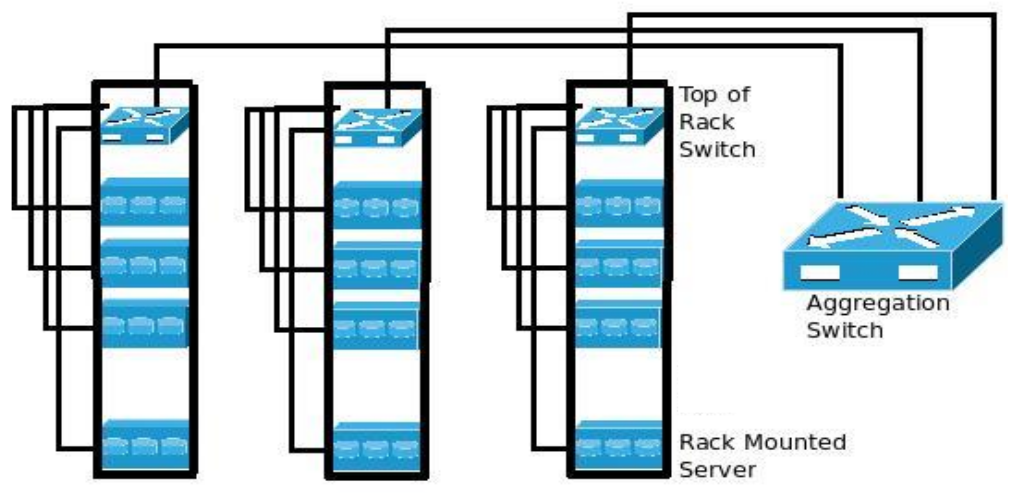
\includegraphics[width=7cm]{img/dcStruct}
\end{tabular}

\subsection{Traffic}

\paragraph{Internal traffic}

Internal traffic (East-west) is clearly a critical component compared
to external traffic (North-south).
\begin{center}
    \begin{tabular}{m{7cm}m{7cm}}

        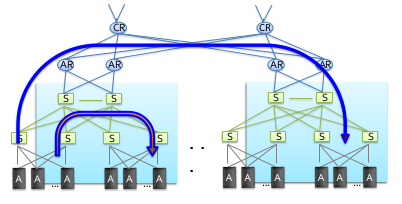
\includegraphics[width=7cm]{img/internalCrit}
        &
        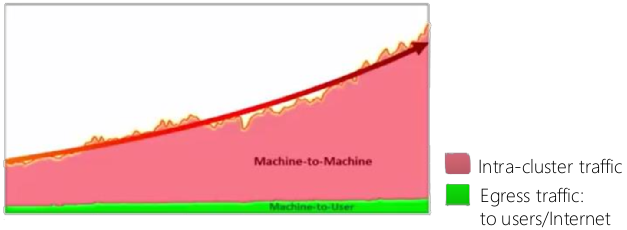
\includegraphics[width=7cm]{img/internalTraffic}
    \end{tabular}
\end{center}

\subsubsection{Solutions}

\begin{tabular}{m{12cm}m{4cm}}
    The goal is to allow each server to talk to any other server at its full access
    link rate.
    We can see the DC as a giant switch between server.
    &
    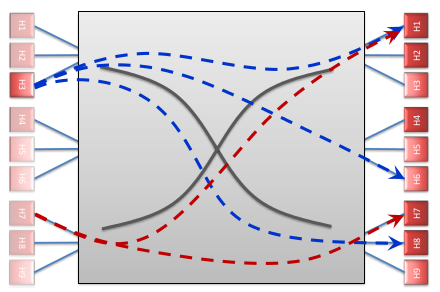
\includegraphics[width=3cm]{img/giant}
\end{tabular}

\begin{itemize}
    \item \textbf{Full Bisection Bandwith }: it's the \textit{scale up } approach.

        \begin{tabular}{m{11cm}m{7cm}}
            A traditional tree topology is really expensive
            because it requires a lot of switch with high bandwidth.
            &
            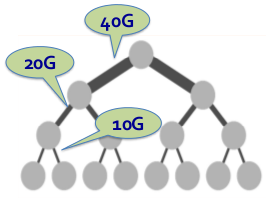
\includegraphics[width=3cm]{img/FBBW}
        \end{tabular}

        \paragraph{Oversubscription}
        A solution is to provision less
        than full Bisection Bandwidth because we can reasonably say
        that all server will know talk with all server simultaneously. 


    \item \textbf{Fat Tree}: it's the \textit{scale out} approach.

        \begin{tabular}{m{11cm}m{7cm}}
            Fat tree offers high bisection bandwidth but
            the system must be to exploit this available capacity:
            \begin{itemize}
                \item Routing must use all path
                \item Transport protocol must fill into all pipe
            \end{itemize}

            Note that this topology only require 10Gb/s links.
            &
            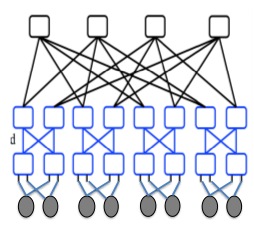
\includegraphics[width=3cm]{img/fattree}
        \end{tabular}
\end{itemize}

\subsection{Network stack}


\paragraph{Models}
Traditional \textbf{TCP} enforce \textit{per-flow min/max fairness}, but
Data center operators want to enforce other models such
as tenant-based or deadline-based.

\paragraph{Low latency}
\begin{itemize}
    \item 55\% of flow $<100KB$ $\Rightarrow$ Delay-sensitive
        So low latency is \textbf{critical}!
    \item 5\% of flow $>10MB$ $\Rightarrow$ Throughput-sensitive
\end{itemize}

\begin{center}
    \begin{tabular}{cc}
        High throughput & Low latency\\
        \hline
        Deep queue at switches& Shallow queues at switches \\
        which increase delays & which
        is bad for burst and throughput\\
    \end{tabular}
\end{center}

The goal is to have in DC low queue occupancy (to achieve
low RRTs within DC approache $1µs$) and high throughput.


\subsubsection{Solutions}
\begin{itemize}
    \item \textbf{DC-TCP} which use \textbf{Explicit Congestion Notification (ECN)} 
        \begin{enumerate}
            \item React early and quickly by using ECN which avoid large
                buildup in queue and allow low latency!

                \paragraph{Switch} If queue length > $k$ set ECN bit

            \item React in proportion to the extend of congestion, not
                in presence.

                \paragraph{Sender} Maintain running average of \textbf{fraction
                of packets marked} ($\alpha$)
                $$ alpha = (1-g) \alpha + g \frac{\# marked ACK}{\# ACK} $$
                and adapts the window based on $\alpha$
                $$ W = (1-\frac{\alpha}{2}) W$$
        \end{enumerate}

    \item \textbf{pFabric}: use priorities
        \begin{enumerate}
            \item Packets carry a single priority number.

                priority = remaining flow size (e.g., \#bytes un-acked)

            \item Switches have small queues (10 packets), send highest
                priority and drop lowest priority

            \item Server (re)transmit aggressively it means at full link rate
                and drop transmission rate only under extreme loss (timeout).
        \end{enumerate}
\end{itemize}

\paragraph{Flow Completion time (FCT)}: is
the time from when flow started at the sender, to when all
packets in the flow were received at the receiver.
\paragraph{Pfabric} With DCTCP, small flow are delayed by big ones. To
handel that:
\begin{itemize}
	\item Packets carry a single priority number representing the remaining flow size.
	\item Switches send the packet with highest priority and drop the lowest
	priority packet
	\item Servers transmit/retransmit at full link rate and decrease transmission
	rate only under extreme loss (typically timeouts)
\end{itemize}
assigning priority number to packet. 
\begin{center}
    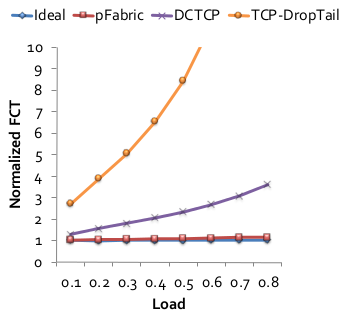
\includegraphics[width=8cm]{img/fct}
\end{center}

\subsection{Management}

\begin{description}
    \item[Data plane]: 
        \begin{tabular}{m{8cm}m{3cm}}
            process packet by using local forwarding state and packet header.
            &
            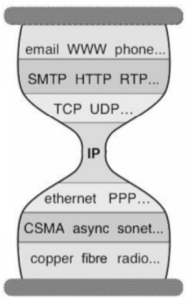
\includegraphics[width=2cm]{img/app}
        \end{tabular}
    \item[Control plane]: Compute forwarding state.

        Actually, we have a protocol which solve
        \begin{itemize}
            \item Consistent with particular low-level hardware/software
            \item  Based on entire network topology
            \item  For all routers/switches (i.e., must configure each one)
        \end{itemize}

        But it's too much, and \textbf{SDN} allow to perform some abstraction.
\end{description}

\subsubsection{Software Defined Network (SDN)}
\begin{center}
    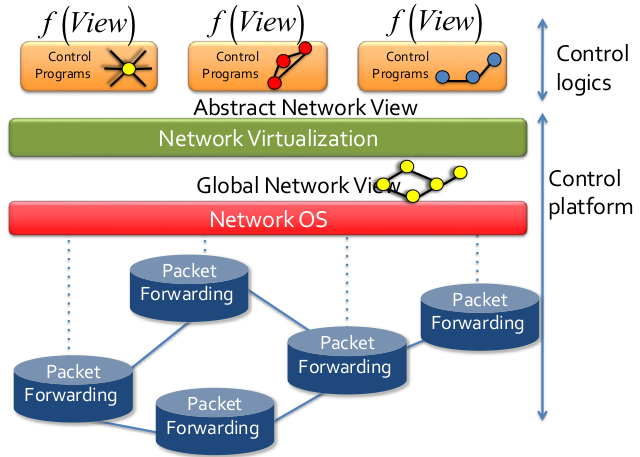
\includegraphics[width=8cm]{img/SDN}
\end{center}

\subsubsection{Open Flow}
is a protocol for remotely controlling the forwarding table of a switch or
router which is one element of SDN.

\begin{tabular}{m{8cm}m{8cm}}
    \begin{itemize}
        \item Message between controller and switches 
            (Synchronous: Stats, Flow-mods, Asynchronous: Packet-in)
        \item Abstract hardware details
        \item  Allows direct control over forwarding table
    \end{itemize}
    &
    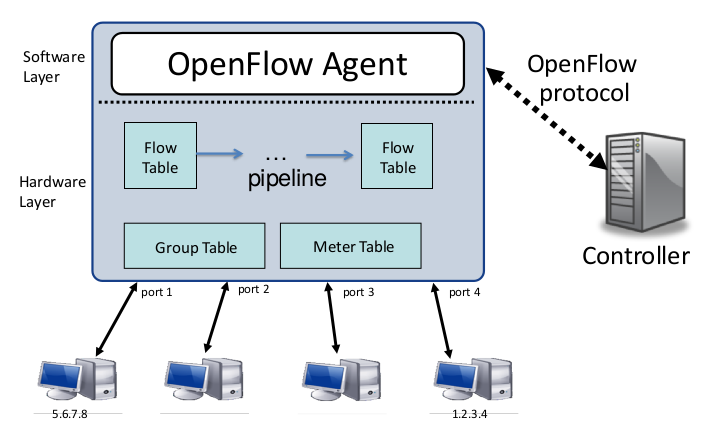
\includegraphics[width=9cm]{img/openflow}
\end{tabular}

\begin{table}[ht!]
	\centering
	\begin{tabular}{|c|l|}
	\hline
	Match field & To match against packet. These consist of the ingress port 
	and packet headers\\
	\hline
	Priority & Matching precedence of the flow entry\\
	\hline
	Counters & e.g. packet and byte counters\\
	\hline
	Instructions & Determine action set or pipeline processing\\
	\hline
	Timeouts & Maximum amount of time or idle time before flow is expired by
	the switch\\
	\hline
	Cookies & Opaque data value chosen by the controller. Not used when
	processing packets.\\
	\hline
	\end{tabular}
	\caption{Flow table entries}
\end{table}

\begin{table}[ht!]
\begin{tabular}{|c|c|c|c|c|c|c|c|c|c|c|c|}
	\hline
	Switch&VLAN&VLAN&MAC&MAC&Eth&IP&IP&IP&IP&L4&L4\\
	Port&ID&pcp&src&dst&type&src&dst&Tos&Prot&sport&dport\\
	\hline
\end{tabular}
\caption{match fields}
\end{table}
\begin{table}[ht!]
	\centering
	\begin{tabular}{|c|c|l|}
	\hline
	Message&Direction&Description\\
	\hline
	Packet-In & Switch$\to$Controller & Transfer the control of the packet to the 
	controller.\\
	&& Packet-in events can be configured to buffer packets.\\
	\hline
	Packet-Out & Controller $\to$ Switch & Instruct switch to send a packet out 
	of a specified port.\\
	&& Send in response to Packet-in messages.\\
	\hline
	Modify-State & Controller$\to$ Switch & Add,delete and modify flow/group entries
	in the flow tables\\
	&& and to set switch port properties.\\
	\hline
	Flow-Removed & Switch $\to$ Controller & Inform the controller about the removal
	of a flow entry \\
	&&from a flow table.\\
	\hline
	\end{tabular}
	\caption{messages exchanged in openFlow}
\end{table}

%TODO improvement from 89 for 08


